\documentclass[a4paper]{article}

%% Language and font encodings
\usepackage[english]{babel}
\usepackage[utf8x]{inputenc}
\usepackage[T1]{fontenc}

%% Sets page size and margins
\usepackage[a4paper,top=3cm,bottom=2cm,left=3cm,right=3cm,marginparwidth=1.75cm]{geometry}

%% Useful packages
\usepackage{amsmath}

\usepackage{graphicx}
\usepackage{listings}
\graphicspath{{./images/}}
\usepackage{tikz}
\usetikzlibrary{arrows}

\usepackage[colorinlistoftodos]{todonotes}
\usepackage[colorlinks=true, allcolors=blue]{hyperref}
\usepackage{xfrac}

\title{Your Paper}
\author{You}

\begin{document}
\maketitle

\section{Introduction}

The goal of this report is to illustrate the work done on a FFT simulator in for the CompMeth course in EURECOM.
The functions developed are able to compute the FFT of a given signal, changing the input signal type, amplitude, number of points and some other parameters that will be described later.

\section{Code Explanation}
\subsection{taus.c}
The purpose of this file is to generate random variable starting from a seed. This seed could be either fixed or a randomly generated value.
\paragraph{modifications:}
As it was, the seed was generated from the current system time, down to a precision of 1 second. This is not exactly good as two consecutive simulations could run in less than one second and, as a consequence, show some correlation. This is the reason why now the random seed is initialized down to a precision of 1 microsecond.
Also, in order to have a full deterministic behavior, another initialization function is able to set the seed to a fixed value.

\subsection{rangen\_double.c}
This is used to generated normally distributed random value trough the function \textit{gaussdouble}.
\paragraph{modifications:}
This piece of code was originally not working because it was developed for a 32-bit machine. Fixing the data types solved this issue.

\subsection{complex.h}
This file contains the definitions of data types used in the entire project. These can be double precision floating point numbers, 32-bit integers or 16-bit integers.
\paragraph{modifications:}
Like the previous file, this was not fully portable too, due to machine-dependent data types. Setting \textit{int32\_t} and \textit{int16\_t} should fix this portability issue for any machine. A comparison between the original and modified code can be found in Listings \ref{CODE:CMXO},\ref{CODE:CMXM}.

\subsection{fixed\_point.c}
Here we define the functions used to compute fixed point saturated addition and multiplication. These functions are available both in a 16-bit and 25-bit version.
\paragraph{modifications:}
Nothing was changed here with the exception of data types.

\subsection{fft.c}
This is the main core of the application, where all the processing of the FFT is done. Each function will be separately covered in this section, together with some brief explanation of their meaning in the overall FFT computation. 


\subsubsection{Twiddle factor}
The functions:
\begin{itemize}
	\item void twiddle(struct complex *W, int N, double stuff)
	\item void twiddle\_fixed(struct complex16 *W, int N, double stuff)         
	\item void twiddle\_fixed\_Q17(struct complex32 *W, int N, double stuff)
\end{itemize}
Are used to compute the twiddle factor. As the prototype indicates, each function is required whether we are using floating points, Q15 or Q24 representations.\\
Following these formula, it's straightforward to understand the computations done in this function and the role of the \textit{stuff} parameter.

\begin{equation}\label{eq:FFT}
X_k = \frac{1}{\sqrt{N}}\sum_{n=0}^{N-1} x_k W_N^{kn}
\end{equation}
$$W_N^{kn} = e^{\frac{-j2\pi kn}{N}} = \cos{(2\pi kn)} - j\sin{(2\pi kn)}$$
$$\mathit{stuff} = kn$$

\paragraph{modifications:}
At the beginning, only the floating point twiddle factor function was present.
The code can be found at the end of this document in Listing \ref{CODE:TWID}

\paragraph{quantization:}
As can be seen in the code, in the fixed point version of the function, a scaling factor is needed to convert from floating to fixed point. (i.e. $\pm32767.0$ for 16-bit).
The range for a Q15 fixed point number goes from $-1$ to $1-2^{-15}$, as a consequence, it is intrinsically not possible to represent exactly the number 1.\\
Radix-4 twiddle factors have the characteristic that the real part ranges from 0 to 1, and the imaginary part from 0 to -1.
The programmer is left with two options: either produce an unbiased result, using $\pm32767.0$, or use $-32768.0$ only for imaginary part and $+32767.0$ for the real part.\\
Trying both of them led to a slightly better result for the biased version, so it was the one left in the code.\\\\
Another important choice is between rounding and truncation. The C standard for typecasting is truncation, thus in order to produce a rounded value it would be necessary to add $\pm0.5$ to the final result before casting.

\subsubsection{Coefficients reordering}
The following functions are needed because after the recursion of the radix 4 FFT butterfly, the coefficients are shuffled in a precise pattern. An simple example of a 16 points radix 4 butterfly can be seen in the following image.\\ 
Again there are three functions used depending on the data type:
\begin{itemize}
	\item bit\_r4\_reorder(struct complex *W, int N)
	\item bit\_r4\_reorder\_fixed\_Q15(struct complex16 *W, int N)
	\item bit\_r4\_reorder\_fixed\_Q24(struct complex32 *W, int N)
\end{itemize}


\tikzstyle{n}= [circle, fill, minimum size=4pt,inner sep=0pt, outer sep=0pt]
\tikzstyle{mul} = [circle,draw,inner sep=-1pt]

% Define two helper counters
\newcounter{x}\newcounter{y}
\begin{tikzpicture}[yscale=0.5, xscale=1.2, node distance=0.4cm, auto]
	% The strategy is to create nodes with names: N-column-row
	% Input nodes are named N-0-0 ... N-0-15
	% Output nodes are named N-10-0 ... N-10-15
	
	% Draw inputs
	\foreach \y in {0,...,15}
		\node[n, pin={[pin edge={latex'-,black}]left:$x(\y)$}]
			(N-0-\y) at (0,-\y) {};
			
	% draw x nodes
	\foreach \y / \x in {0/5,1/7,2/9,3/11}{
		\node[mul] (N-2-\y) at (2,-\x+0.5) {${\times}$};
	}
\foreach \y / \x in {0/2,1/6,2/10,3/14}{
	\node[mul] (N-5-\y) at (5.5,-\x+0.5) {${\times}$};
}
		
	\foreach \y in {0,...,15}
	\node[n]
	(N-4-\y) at (4,-\y) {};
	
	% Draw outputs
	\foreach \y / \idx in {	0/0,1/4,2/8,3/12,4/1,5/5,6/9,7/13,8/2,9/6,10/10,11/14,12/3,13/7,14/11,15/15}
		\node[n, pin={[pin edge={-latex',black}]right:$X(\idx)$}]
			(N-7-\y) at (7,-\y) {};
			
	\foreach \sourcey / \desty in {0/0,1/1,2/2,3/3}{
		\path (N-0-\sourcey.east) edge[-] (N-2-\desty.west);
		\path (N-2-\desty.east) edge[-] (N-4-\sourcey.west);
	}
	\foreach \sourcey / \desty in {4/0,5/1,6/2,7/3}{
		\path (N-0-\sourcey.east) edge[-] (N-2-\desty.west);
		\path (N-2-\desty.east) edge[-] (N-4-\sourcey.west);
	}
	\foreach \sourcey / \desty in {8/0,9/1,10/2,11/3}{
		\path (N-0-\sourcey.east) edge[-] (N-2-\desty.west);
		\path (N-2-\desty.east) edge[-] (N-4-\sourcey.west);
	}
	\foreach \sourcey / \desty in {12/0,13/1,14/2,15/3}{
		\path (N-0-\sourcey.east) edge[-] (N-2-\desty.west);
		\path (N-2-\desty.east) edge[-] (N-4-\sourcey.west);
	}


	\foreach \sourcey / \desty in {0/0,1/0,2/0,3/0}{
		\path (N-4-\sourcey.east) edge[-] (N-5-\desty.west);
		\path (N-5-\desty.east) edge[-] (N-7-\sourcey.west);
	}
	\foreach \sourcey / \desty in {4/1,5/1,6/1,7/1}{
		\path (N-4-\sourcey.east) edge[-] (N-5-\desty.west);
		\path (N-5-\desty.east) edge[-] (N-7-\sourcey.west);
	}
	\foreach \sourcey / \desty in {8/2,9/2,10/2,11/2}{
		\path (N-4-\sourcey.east) edge[-] (N-5-\desty.west);
		\path (N-5-\desty.east) edge[-] (N-7-\sourcey.west);
	}
	\foreach \sourcey / \desty in {12/3,13/3,14/3,15/3}{
		\path (N-4-\sourcey.east) edge[-] (N-5-\desty.west);
		\path (N-5-\desty.east) edge[-] (N-7-\sourcey.west);
	}
	\end{tikzpicture}
	
	\paragraph{modifications}
	A weird bug was discovered and fixed in the fixed point version of the function. As can be seen in the two code listings, the original code was applying the scaling only to those coefficients that were swapped. Fixing this bug strongly improved the output SNR, especially in the low dB input where the scaling is more likely to be executed at the reordering phase.
	A comparison between the two codes can be found in Listings \ref{CODE:REORDERO},\ref{CODE:REORDERM}.


\subsubsection{Radix 4}
\label{SUB:Radix4}
This is the core function where the FFT coefficients are actually calculated. The function is recursive, and calls itself back until no more splitting is possible(when there is only one butterfly left), every time cutting the number of iterations by \sfrac{1}{4}.
\paragraph{shifting}
At each stage, the input data might be right shifted by a scale value, ranging from 0 to $log_2(\sqrt{N})$. This is because, according to (\ref{eq:FFT}), final coefficients must be divided by a factor $\sqrt{N}$. This shift can be split in all the stages of the Radix-4 FFT in order to achieve the maximum possible precision with the least number of saturations.
\begin{itemize}
	\item radix4(struct complex *x, int N)
	\item void radix4\_fixed\_Q15(struct complex16 *x, int N, uns char *scale, uns char stage)
	\item void radix4\_fixed\_Q24(struct complex32 *x, int N, uns char *scale, uns char stage)
\end{itemize}
As for the other functions this one is also present three times, depending on input data type.
\paragraph{modifications}
Other than constructing the functions for fixed point arithmetics, a simple control on the twiddle factor was developed in order to skip multiplications when the twiddle factor is equal to 1. This would slightly reduce computation time and, more important, avoid possible precision losses.
The code of the 16-bit fixed point version can be found in Listing \ref{CODE:RADIX4}

\subsubsection{QAM input}
This helper function is called in the two cases when PSK or QAM input is needed, it will simply fill the input vector with the right numbers. This function was left untouched.
\subsubsection{distortion test}
The purpose of this function is to run a single simulation of an FFT both in double precision arithmetic and one between 16-bit or 25-bit fixed point arithmetic and produce an output SNR value between the two.
The formula used to calculate the SNR is:

$$\mathit{SNR} = 10\log_{10}{\left(\frac{\sum_{n=0}^{N-1}{|X_n^f - X_n^d|^2}}{\sum_{n=0}^{N-1}{|X_n^f|^2}}\right)}$$

Where $X_n^f$ is the n-th value of the floating point FFT and $X_n^d$ is the fixed point version of the same value.\\\\
Also at the end of the computation, if the current SNR is better than the stored maximum, that value is updated(\textit{maxSNR}) and the current scaling is saved(\textit{maxscale}).\\\\
As shown in the prototype, many other parameters are required. Most of them are pretty self explained by the comments.
One parameter worth mentioning is \textit{test}. It is an integer value passed from the calling function which is used to generate the input signal according to the following scheme:
\begin{description}
	\item[0 $\rightarrow$] fixed frequency cosine signal
	\item[1 $\rightarrow$] PSK white noise signal
	\item[2 $\rightarrow$] 16QAM white noise signal
	\item[3 $\rightarrow$] Gaussian white noise signal
\end{description}

Most of the code in this function was left untouched, with the exception of the extension to Q24 fixed point structure, leading to the inclusion of \textit{data\_t} and \textit{shift} parameters.
The first is a simple selector of data type, while the latter will be discussed later in \ref{25BIT}.

\begin{lstlisting}
void fft_distortion_test(
int N,                              // dimension of FFT under test 
char test,                          // type of test
double input_dB,                    // strength of input
char *scale,                        // pointer to scaling schedule
double *maxSNR,                     // pointer best signal-to-noise ratio
char *maxscale,                     // pointer to best scaling schedule
struct complex *data,               // pointer to floating point data vector
struct complex16 *data16,           // pointer to Q15 data vector
struct complex32 *data32,           // pointer to Q17 data vector
int data_t,                         // 16 or 25 bit input
int shift)                          // 25-bit only pre/post shift

\end{lstlisting}

\subsubsection{main}
The purpose of the main function, other than obviously interfacing with the user and extrapolate input parameters, is to actually launch the executions of the simulation.
Considering that one strong factor of the output quality is the scaling schedule(previously mentioned in \ref{SUB:Radix4}), the main function simply tries all the possible combinations in an exhaustive manner and prints out only the best one. This is also the reason why the final execution time is so long, the complexity of the search is: $$\frac{(2n)!}{(n!)^2}$$
where:
$$n = log_2{\sqrt{N}}$$
\pagebreak
\section{Results}
As suggested in the instruction, it is interesting to see the input signal strength versus the signal-to-distortion ratio to find the practical dynamic range.
As there are no given numbers to use to decide the acceptable SNR threshold, a 50dB value has been chosen.

\subsection{Calculate the Input Dynamic Range}
\begin{figure}
	\centering
	\resizebox{1.0\textwidth}{!}{% GNUPLOT: LaTeX picture with Postscript
\begingroup
  \makeatletter
  \providecommand\color[2][]{%
    \GenericError{(gnuplot) \space\space\space\@spaces}{%
      Package color not loaded in conjunction with
      terminal option `colourtext'%
    }{See the gnuplot documentation for explanation.%
    }{Either use 'blacktext' in gnuplot or load the package
      color.sty in LaTeX.}%
    \renewcommand\color[2][]{}%
  }%
  \providecommand\includegraphics[2][]{%
    \GenericError{(gnuplot) \space\space\space\@spaces}{%
      Package graphicx or graphics not loaded%
    }{See the gnuplot documentation for explanation.%
    }{The gnuplot epslatex terminal needs graphicx.sty or graphics.sty.}%
    \renewcommand\includegraphics[2][]{}%
  }%
  \providecommand\rotatebox[2]{#2}%
  \@ifundefined{ifGPcolor}{%
    \newif\ifGPcolor
    \GPcolortrue
  }{}%
  \@ifundefined{ifGPblacktext}{%
    \newif\ifGPblacktext
    \GPblacktextfalse
  }{}%
  % define a \g@addto@macro without @ in the name:
  \let\gplgaddtomacro\g@addto@macro
  % define empty templates for all commands taking text:
  \gdef\gplbacktext{}%
  \gdef\gplfronttext{}%
  \makeatother
  \ifGPblacktext
    % no textcolor at all
    \def\colorrgb#1{}%
    \def\colorgray#1{}%
  \else
    % gray or color?
    \ifGPcolor
      \def\colorrgb#1{\color[rgb]{#1}}%
      \def\colorgray#1{\color[gray]{#1}}%
      \expandafter\def\csname LTw\endcsname{\color{white}}%
      \expandafter\def\csname LTb\endcsname{\color{black}}%
      \expandafter\def\csname LTa\endcsname{\color{black}}%
      \expandafter\def\csname LT0\endcsname{\color[rgb]{1,0,0}}%
      \expandafter\def\csname LT1\endcsname{\color[rgb]{0,1,0}}%
      \expandafter\def\csname LT2\endcsname{\color[rgb]{0,0,1}}%
      \expandafter\def\csname LT3\endcsname{\color[rgb]{1,0,1}}%
      \expandafter\def\csname LT4\endcsname{\color[rgb]{0,1,1}}%
      \expandafter\def\csname LT5\endcsname{\color[rgb]{1,1,0}}%
      \expandafter\def\csname LT6\endcsname{\color[rgb]{0,0,0}}%
      \expandafter\def\csname LT7\endcsname{\color[rgb]{1,0.3,0}}%
      \expandafter\def\csname LT8\endcsname{\color[rgb]{0.5,0.5,0.5}}%
    \else
      % gray
      \def\colorrgb#1{\color{black}}%
      \def\colorgray#1{\color[gray]{#1}}%
      \expandafter\def\csname LTw\endcsname{\color{white}}%
      \expandafter\def\csname LTb\endcsname{\color{black}}%
      \expandafter\def\csname LTa\endcsname{\color{black}}%
      \expandafter\def\csname LT0\endcsname{\color{black}}%
      \expandafter\def\csname LT1\endcsname{\color{black}}%
      \expandafter\def\csname LT2\endcsname{\color{black}}%
      \expandafter\def\csname LT3\endcsname{\color{black}}%
      \expandafter\def\csname LT4\endcsname{\color{black}}%
      \expandafter\def\csname LT5\endcsname{\color{black}}%
      \expandafter\def\csname LT6\endcsname{\color{black}}%
      \expandafter\def\csname LT7\endcsname{\color{black}}%
      \expandafter\def\csname LT8\endcsname{\color{black}}%
    \fi
  \fi
    \setlength{\unitlength}{0.0500bp}%
    \ifx\gptboxheight\undefined%
      \newlength{\gptboxheight}%
      \newlength{\gptboxwidth}%
      \newsavebox{\gptboxtext}%
    \fi%
    \setlength{\fboxrule}{0.5pt}%
    \setlength{\fboxsep}{1pt}%
\begin{picture}(5040.00,3772.00)%
    \gplgaddtomacro\gplbacktext{%
      \csname LTb\endcsname%
      \put(396,594){\makebox(0,0)[r]{\strut{}\footnotesize{$0$}}}%
      \csname LTb\endcsname%
      \put(396,909){\makebox(0,0)[r]{\strut{}\footnotesize{$10$}}}%
      \csname LTb\endcsname%
      \put(396,1223){\makebox(0,0)[r]{\strut{}\footnotesize{$20$}}}%
      \csname LTb\endcsname%
      \put(396,1538){\makebox(0,0)[r]{\strut{}\footnotesize{$30$}}}%
      \csname LTb\endcsname%
      \put(396,1853){\makebox(0,0)[r]{\strut{}\footnotesize{$40$}}}%
      \csname LTb\endcsname%
      \put(396,2167){\makebox(0,0)[r]{\strut{}\footnotesize{$50$}}}%
      \csname LTb\endcsname%
      \put(396,2482){\makebox(0,0)[r]{\strut{}\footnotesize{$60$}}}%
      \csname LTb\endcsname%
      \put(396,2796){\makebox(0,0)[r]{\strut{}\footnotesize{$70$}}}%
      \csname LTb\endcsname%
      \put(396,3111){\makebox(0,0)[r]{\strut{}\footnotesize{$80$}}}%
      \csname LTb\endcsname%
      \put(528,374){\makebox(0,0){\strut{}\footnotesize{$-60$}}}%
      \csname LTb\endcsname%
      \put(1192,374){\makebox(0,0){\strut{}\footnotesize{$-50$}}}%
      \csname LTb\endcsname%
      \put(1856,374){\makebox(0,0){\strut{}\footnotesize{$-40$}}}%
      \csname LTb\endcsname%
      \put(2520,374){\makebox(0,0){\strut{}\footnotesize{$-30$}}}%
      \csname LTb\endcsname%
      \put(3183,374){\makebox(0,0){\strut{}\footnotesize{$-20$}}}%
      \csname LTb\endcsname%
      \put(3847,374){\makebox(0,0){\strut{}\footnotesize{$-10$}}}%
      \csname LTb\endcsname%
      \put(4511,374){\makebox(0,0){\strut{}\footnotesize{$0$}}}%
    }%
    \gplgaddtomacro\gplfronttext{%
      \csname LTb\endcsname%
      \put(88,1852){\rotatebox{-270}{\makebox(0,0){\strut{}\footnotesize{SNR [dB]}}}}%
      \put(2519,154){\makebox(0,0){\strut{}\footnotesize{input [dB]}}}%
      \put(2519,3441){\makebox(0,0){\strut{}\shortstack{Input Dynamic Range\\16QAM Q1.15 FFT256}}}%
    }%
    \gplbacktext
    \put(0,0){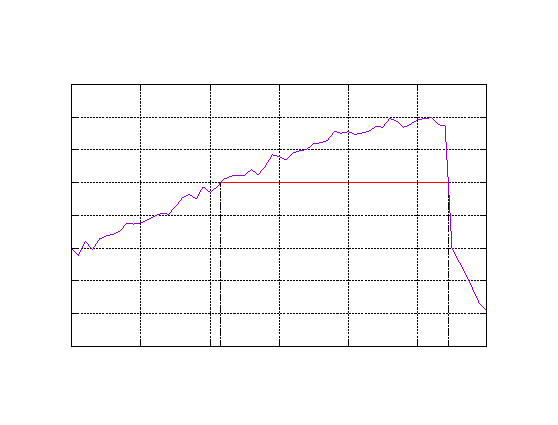
\includegraphics{dyn_range}}%
    \gplfronttext
  \end{picture}%
\endgroup
}
	%%% GNUPLOT: LaTeX picture with Postscript
\begingroup
  \makeatletter
  \providecommand\color[2][]{%
    \GenericError{(gnuplot) \space\space\space\@spaces}{%
      Package color not loaded in conjunction with
      terminal option `colourtext'%
    }{See the gnuplot documentation for explanation.%
    }{Either use 'blacktext' in gnuplot or load the package
      color.sty in LaTeX.}%
    \renewcommand\color[2][]{}%
  }%
  \providecommand\includegraphics[2][]{%
    \GenericError{(gnuplot) \space\space\space\@spaces}{%
      Package graphicx or graphics not loaded%
    }{See the gnuplot documentation for explanation.%
    }{The gnuplot epslatex terminal needs graphicx.sty or graphics.sty.}%
    \renewcommand\includegraphics[2][]{}%
  }%
  \providecommand\rotatebox[2]{#2}%
  \@ifundefined{ifGPcolor}{%
    \newif\ifGPcolor
    \GPcolortrue
  }{}%
  \@ifundefined{ifGPblacktext}{%
    \newif\ifGPblacktext
    \GPblacktextfalse
  }{}%
  % define a \g@addto@macro without @ in the name:
  \let\gplgaddtomacro\g@addto@macro
  % define empty templates for all commands taking text:
  \gdef\gplbacktext{}%
  \gdef\gplfronttext{}%
  \makeatother
  \ifGPblacktext
    % no textcolor at all
    \def\colorrgb#1{}%
    \def\colorgray#1{}%
  \else
    % gray or color?
    \ifGPcolor
      \def\colorrgb#1{\color[rgb]{#1}}%
      \def\colorgray#1{\color[gray]{#1}}%
      \expandafter\def\csname LTw\endcsname{\color{white}}%
      \expandafter\def\csname LTb\endcsname{\color{black}}%
      \expandafter\def\csname LTa\endcsname{\color{black}}%
      \expandafter\def\csname LT0\endcsname{\color[rgb]{1,0,0}}%
      \expandafter\def\csname LT1\endcsname{\color[rgb]{0,1,0}}%
      \expandafter\def\csname LT2\endcsname{\color[rgb]{0,0,1}}%
      \expandafter\def\csname LT3\endcsname{\color[rgb]{1,0,1}}%
      \expandafter\def\csname LT4\endcsname{\color[rgb]{0,1,1}}%
      \expandafter\def\csname LT5\endcsname{\color[rgb]{1,1,0}}%
      \expandafter\def\csname LT6\endcsname{\color[rgb]{0,0,0}}%
      \expandafter\def\csname LT7\endcsname{\color[rgb]{1,0.3,0}}%
      \expandafter\def\csname LT8\endcsname{\color[rgb]{0.5,0.5,0.5}}%
    \else
      % gray
      \def\colorrgb#1{\color{black}}%
      \def\colorgray#1{\color[gray]{#1}}%
      \expandafter\def\csname LTw\endcsname{\color{white}}%
      \expandafter\def\csname LTb\endcsname{\color{black}}%
      \expandafter\def\csname LTa\endcsname{\color{black}}%
      \expandafter\def\csname LT0\endcsname{\color{black}}%
      \expandafter\def\csname LT1\endcsname{\color{black}}%
      \expandafter\def\csname LT2\endcsname{\color{black}}%
      \expandafter\def\csname LT3\endcsname{\color{black}}%
      \expandafter\def\csname LT4\endcsname{\color{black}}%
      \expandafter\def\csname LT5\endcsname{\color{black}}%
      \expandafter\def\csname LT6\endcsname{\color{black}}%
      \expandafter\def\csname LT7\endcsname{\color{black}}%
      \expandafter\def\csname LT8\endcsname{\color{black}}%
    \fi
  \fi
    \setlength{\unitlength}{0.0500bp}%
    \ifx\gptboxheight\undefined%
      \newlength{\gptboxheight}%
      \newlength{\gptboxwidth}%
      \newsavebox{\gptboxtext}%
    \fi%
    \setlength{\fboxrule}{0.5pt}%
    \setlength{\fboxsep}{1pt}%
\begin{picture}(5040.00,3772.00)%
    \gplgaddtomacro\gplbacktext{%
      \csname LTb\endcsname%
      \put(396,594){\makebox(0,0)[r]{\strut{}\footnotesize{$0$}}}%
      \csname LTb\endcsname%
      \put(396,954){\makebox(0,0)[r]{\strut{}\footnotesize{$10$}}}%
      \csname LTb\endcsname%
      \put(396,1313){\makebox(0,0)[r]{\strut{}\footnotesize{$20$}}}%
      \csname LTb\endcsname%
      \put(396,1673){\makebox(0,0)[r]{\strut{}\footnotesize{$30$}}}%
      \csname LTb\endcsname%
      \put(396,2032){\makebox(0,0)[r]{\strut{}\footnotesize{$40$}}}%
      \csname LTb\endcsname%
      \put(396,2392){\makebox(0,0)[r]{\strut{}\footnotesize{$50$}}}%
      \csname LTb\endcsname%
      \put(396,2751){\makebox(0,0)[r]{\strut{}\footnotesize{$60$}}}%
      \csname LTb\endcsname%
      \put(396,3111){\makebox(0,0)[r]{\strut{}\footnotesize{$70$}}}%
      \csname LTb\endcsname%
      \put(528,374){\makebox(0,0){\strut{}\footnotesize{$-60$}}}%
      \csname LTb\endcsname%
      \put(1192,374){\makebox(0,0){\strut{}\footnotesize{$-50$}}}%
      \csname LTb\endcsname%
      \put(1856,374){\makebox(0,0){\strut{}\footnotesize{$-40$}}}%
      \csname LTb\endcsname%
      \put(2520,374){\makebox(0,0){\strut{}\footnotesize{$-30$}}}%
      \csname LTb\endcsname%
      \put(3183,374){\makebox(0,0){\strut{}\footnotesize{$-20$}}}%
      \csname LTb\endcsname%
      \put(3847,374){\makebox(0,0){\strut{}\footnotesize{$-10$}}}%
      \csname LTb\endcsname%
      \put(4511,374){\makebox(0,0){\strut{}\footnotesize{$0$}}}%
    }%
    \gplgaddtomacro\gplfronttext{%
      \csname LTb\endcsname%
      \put(88,1852){\rotatebox{-270}{\makebox(0,0){\strut{}\footnotesize{SNR [dB]}}}}%
      \put(2519,154){\makebox(0,0){\strut{}\footnotesize{input [dB]}}}%
      \put(2519,3441){\makebox(0,0){\strut{}\shortstack{16-bit Fixed point \\Cosine $f=0.1$ Q1.15}}}%
      \csname LTb\endcsname%
      \put(1188,1196){\makebox(0,0)[r]{\strut{}\tiny{FFT64}}}%
      \csname LTb\endcsname%
      \put(1188,1042){\makebox(0,0)[r]{\strut{}\tiny{FFT256}}}%
      \csname LTb\endcsname%
      \put(1188,888){\makebox(0,0)[r]{\strut{}\tiny{FFT1024}}}%
      \csname LTb\endcsname%
      \put(1188,734){\makebox(0,0)[r]{\strut{}\tiny{FFT4096}}}%
    }%
    \gplbacktext
    \put(0,0){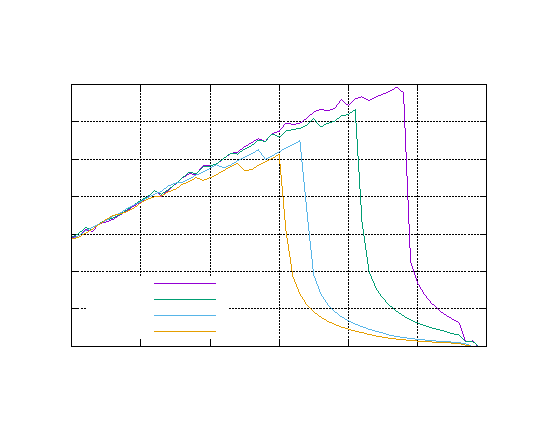
\includegraphics{cosine_DR}}%
    \gplfronttext
  \end{picture}%
\endgroup

	\caption{Input dynamic range calculation.}
	\label{Fig:DYN}
\end{figure}
As show in Figure \ref{Fig:DYN}, calculating the input dynamic range is not difficult. Every input signal shows almost the same behavior: the SNR is roughly increasing linearly with the input dB, while at a certain point there is a sudden drop on the output quality. The input dynamic range is simply the range for which the output is higher than the threshold. In the example it spaces from -38dB to -6dB.
\subsection{Fixed Point Saturation}
\begin{figure}
	\centering
	\resizebox{1.0\textwidth}{!}{% GNUPLOT: LaTeX picture with Postscript
\begingroup
  \makeatletter
  \providecommand\color[2][]{%
    \GenericError{(gnuplot) \space\space\space\@spaces}{%
      Package color not loaded in conjunction with
      terminal option `colourtext'%
    }{See the gnuplot documentation for explanation.%
    }{Either use 'blacktext' in gnuplot or load the package
      color.sty in LaTeX.}%
    \renewcommand\color[2][]{}%
  }%
  \providecommand\includegraphics[2][]{%
    \GenericError{(gnuplot) \space\space\space\@spaces}{%
      Package graphicx or graphics not loaded%
    }{See the gnuplot documentation for explanation.%
    }{The gnuplot epslatex terminal needs graphicx.sty or graphics.sty.}%
    \renewcommand\includegraphics[2][]{}%
  }%
  \providecommand\rotatebox[2]{#2}%
  \@ifundefined{ifGPcolor}{%
    \newif\ifGPcolor
    \GPcolortrue
  }{}%
  \@ifundefined{ifGPblacktext}{%
    \newif\ifGPblacktext
    \GPblacktextfalse
  }{}%
  % define a \g@addto@macro without @ in the name:
  \let\gplgaddtomacro\g@addto@macro
  % define empty templates for all commands taking text:
  \gdef\gplbacktext{}%
  \gdef\gplfronttext{}%
  \makeatother
  \ifGPblacktext
    % no textcolor at all
    \def\colorrgb#1{}%
    \def\colorgray#1{}%
  \else
    % gray or color?
    \ifGPcolor
      \def\colorrgb#1{\color[rgb]{#1}}%
      \def\colorgray#1{\color[gray]{#1}}%
      \expandafter\def\csname LTw\endcsname{\color{white}}%
      \expandafter\def\csname LTb\endcsname{\color{black}}%
      \expandafter\def\csname LTa\endcsname{\color{black}}%
      \expandafter\def\csname LT0\endcsname{\color[rgb]{1,0,0}}%
      \expandafter\def\csname LT1\endcsname{\color[rgb]{0,1,0}}%
      \expandafter\def\csname LT2\endcsname{\color[rgb]{0,0,1}}%
      \expandafter\def\csname LT3\endcsname{\color[rgb]{1,0,1}}%
      \expandafter\def\csname LT4\endcsname{\color[rgb]{0,1,1}}%
      \expandafter\def\csname LT5\endcsname{\color[rgb]{1,1,0}}%
      \expandafter\def\csname LT6\endcsname{\color[rgb]{0,0,0}}%
      \expandafter\def\csname LT7\endcsname{\color[rgb]{1,0.3,0}}%
      \expandafter\def\csname LT8\endcsname{\color[rgb]{0.5,0.5,0.5}}%
    \else
      % gray
      \def\colorrgb#1{\color{black}}%
      \def\colorgray#1{\color[gray]{#1}}%
      \expandafter\def\csname LTw\endcsname{\color{white}}%
      \expandafter\def\csname LTb\endcsname{\color{black}}%
      \expandafter\def\csname LTa\endcsname{\color{black}}%
      \expandafter\def\csname LT0\endcsname{\color{black}}%
      \expandafter\def\csname LT1\endcsname{\color{black}}%
      \expandafter\def\csname LT2\endcsname{\color{black}}%
      \expandafter\def\csname LT3\endcsname{\color{black}}%
      \expandafter\def\csname LT4\endcsname{\color{black}}%
      \expandafter\def\csname LT5\endcsname{\color{black}}%
      \expandafter\def\csname LT6\endcsname{\color{black}}%
      \expandafter\def\csname LT7\endcsname{\color{black}}%
      \expandafter\def\csname LT8\endcsname{\color{black}}%
    \fi
  \fi
    \setlength{\unitlength}{0.0500bp}%
    \ifx\gptboxheight\undefined%
      \newlength{\gptboxheight}%
      \newlength{\gptboxwidth}%
      \newsavebox{\gptboxtext}%
    \fi%
    \setlength{\fboxrule}{0.5pt}%
    \setlength{\fboxsep}{1pt}%
\begin{picture}(10080.00,3772.00)%
    \gplgaddtomacro\gplbacktext{%
      \csname LTb\endcsname%
      \put(396,594){\makebox(0,0)[r]{\strut{}\footnotesize{$-0.8$}}}%
      \csname LTb\endcsname%
      \put(396,909){\makebox(0,0)[r]{\strut{}\footnotesize{$-0.6$}}}%
      \csname LTb\endcsname%
      \put(396,1223){\makebox(0,0)[r]{\strut{}\footnotesize{$-0.4$}}}%
      \csname LTb\endcsname%
      \put(396,1538){\makebox(0,0)[r]{\strut{}\footnotesize{$-0.2$}}}%
      \csname LTb\endcsname%
      \put(396,1853){\makebox(0,0)[r]{\strut{}\footnotesize{$0$}}}%
      \csname LTb\endcsname%
      \put(396,2167){\makebox(0,0)[r]{\strut{}\footnotesize{$0.2$}}}%
      \csname LTb\endcsname%
      \put(396,2482){\makebox(0,0)[r]{\strut{}\footnotesize{$0.4$}}}%
      \csname LTb\endcsname%
      \put(396,2796){\makebox(0,0)[r]{\strut{}\footnotesize{$0.6$}}}%
      \csname LTb\endcsname%
      \put(396,3111){\makebox(0,0)[r]{\strut{}\footnotesize{$0.8$}}}%
      \csname LTb\endcsname%
      \put(528,374){\makebox(0,0){\strut{}\footnotesize{$0$}}}%
      \csname LTb\endcsname%
      \put(1026,374){\makebox(0,0){\strut{}\footnotesize{$8$}}}%
      \csname LTb\endcsname%
      \put(1524,374){\makebox(0,0){\strut{}\footnotesize{$16$}}}%
      \csname LTb\endcsname%
      \put(2022,374){\makebox(0,0){\strut{}\footnotesize{$24$}}}%
      \csname LTb\endcsname%
      \put(2520,374){\makebox(0,0){\strut{}\footnotesize{$32$}}}%
      \csname LTb\endcsname%
      \put(3017,374){\makebox(0,0){\strut{}\footnotesize{$40$}}}%
      \csname LTb\endcsname%
      \put(3515,374){\makebox(0,0){\strut{}\footnotesize{$48$}}}%
      \csname LTb\endcsname%
      \put(4013,374){\makebox(0,0){\strut{}\footnotesize{$56$}}}%
      \csname LTb\endcsname%
      \put(4511,374){\makebox(0,0){\strut{}\footnotesize{$64$}}}%
    }%
    \gplgaddtomacro\gplfronttext{%
      \csname LTb\endcsname%
      \put(-176,1852){\rotatebox{-270}{\makebox(0,0){\strut{}\footnotesize{$cos(2\pi fi)$}}}}%
      \put(2519,154){\makebox(0,0){\strut{}\footnotesize{$i$}}}%
      \put(2519,3441){\makebox(0,0){\strut{}\shortstack{input\\ $N=64$ $f=0.1$ $dB=-5$}}}%
    }%
    \gplgaddtomacro\gplbacktext{%
      \csname LTb\endcsname%
      \put(5436,594){\makebox(0,0)[r]{\strut{}\footnotesize{$10^{-5}$}}}%
      \csname LTb\endcsname%
      \put(5436,1014){\makebox(0,0)[r]{\strut{}\footnotesize{$10^{-4}$}}}%
      \csname LTb\endcsname%
      \put(5436,1433){\makebox(0,0)[r]{\strut{}\footnotesize{$10^{-3}$}}}%
      \csname LTb\endcsname%
      \put(5436,1853){\makebox(0,0)[r]{\strut{}\footnotesize{$10^{-2}$}}}%
      \csname LTb\endcsname%
      \put(5436,2272){\makebox(0,0)[r]{\strut{}\footnotesize{$10^{-1}$}}}%
      \csname LTb\endcsname%
      \put(5436,2692){\makebox(0,0)[r]{\strut{}\footnotesize{$10^{0}$}}}%
      \csname LTb\endcsname%
      \put(5436,3111){\makebox(0,0)[r]{\strut{}\footnotesize{$10^{1}$}}}%
      \csname LTb\endcsname%
      \put(5568,374){\makebox(0,0){\strut{}\footnotesize{$0$}}}%
      \csname LTb\endcsname%
      \put(6066,374){\makebox(0,0){\strut{}\footnotesize{$8$}}}%
      \csname LTb\endcsname%
      \put(6564,374){\makebox(0,0){\strut{}\footnotesize{$16$}}}%
      \csname LTb\endcsname%
      \put(7062,374){\makebox(0,0){\strut{}\footnotesize{$24$}}}%
      \csname LTb\endcsname%
      \put(7560,374){\makebox(0,0){\strut{}\footnotesize{$32$}}}%
      \csname LTb\endcsname%
      \put(8057,374){\makebox(0,0){\strut{}\footnotesize{$40$}}}%
      \csname LTb\endcsname%
      \put(8555,374){\makebox(0,0){\strut{}\footnotesize{$48$}}}%
      \csname LTb\endcsname%
      \put(9053,374){\makebox(0,0){\strut{}\footnotesize{$56$}}}%
      \csname LTb\endcsname%
      \put(9551,374){\makebox(0,0){\strut{}\footnotesize{$64$}}}%
    }%
    \gplgaddtomacro\gplfronttext{%
      \csname LTb\endcsname%
      \put(4864,1852){\rotatebox{-270}{\makebox(0,0){\strut{}\footnotesize{$|X_n|$}}}}%
      \put(7559,154){\makebox(0,0){\strut{}\footnotesize{$n$}}}%
      \put(7559,3441){\makebox(0,0){\strut{}\shortstack{FFT\\ $N=64$ $f=0.1$ $dB=-5$}}}%
      \csname LTb\endcsname%
      \put(6934,2938){\makebox(0,0)[l]{\strut{}\tiny{FFT64 FP}}}%
      \csname LTb\endcsname%
      \put(6934,2718){\makebox(0,0)[l]{\strut{}\tiny{FFT64 Q1.15 }}}%
      \csname LTb\endcsname%
      \put(6934,2498){\makebox(0,0)[l]{\strut{}\tiny{FFT64 Q11.15}}}%
    }%
    \gplbacktext
    \put(0,0){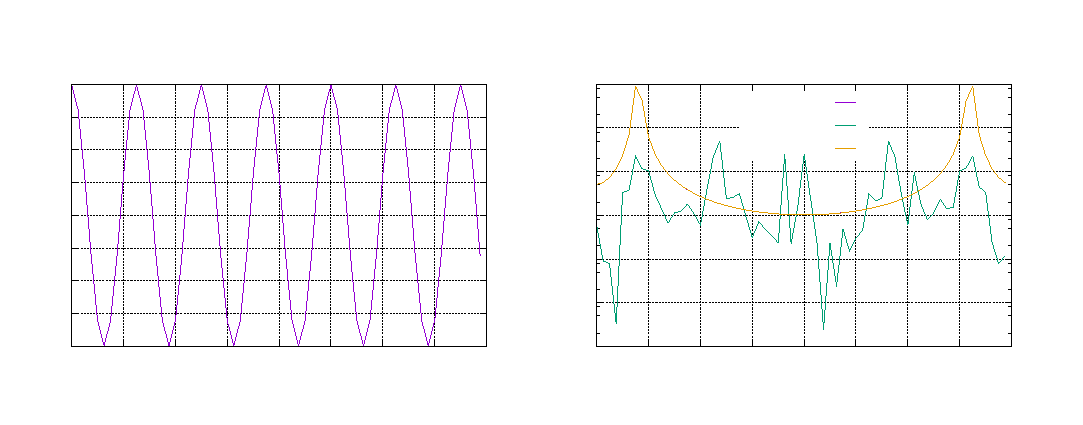
\includegraphics{cosineFFT}}%
    \gplfronttext
  \end{picture}%
\endgroup
}
	\caption{Input dynamic range calculation.}
	\label{Fig:COSINE}
\end{figure}
One particular drawback of fixed point representation is saturation. In our case this particular phenomenon can happen in case of additions for which the result inevitably fall outside of the possible range. Fortunately, as discussed in \ref{SUB:Radix4}, FFT shifting helps to overcome this problem.
However, at some point, even after the maximum scaling applied directly at the input, the output will saturate. Moving to a 25-bit representation could enlarge the input dynamic range and provide good results where the 16-bit reaches its limit.\\\\
Figure \ref{Fig:COSINE} shows on the left the cosine input signal, and on the right the same FFT computed in three different bit representations. At this point signal input strength Q1.15 is no more able to avoid saturations, and the resulting FFT spectrum is unavoidably compromised. Q10.15 instead is still in its dynamic range and provide an almost identical spectrum.
\subsection{FFT Output Comparison}
\begin{figure}
	\centering
	\resizebox{1.0\textwidth}{!}{% GNUPLOT: LaTeX picture with Postscript
\begingroup
  \makeatletter
  \providecommand\color[2][]{%
    \GenericError{(gnuplot) \space\space\space\@spaces}{%
      Package color not loaded in conjunction with
      terminal option `colourtext'%
    }{See the gnuplot documentation for explanation.%
    }{Either use 'blacktext' in gnuplot or load the package
      color.sty in LaTeX.}%
    \renewcommand\color[2][]{}%
  }%
  \providecommand\includegraphics[2][]{%
    \GenericError{(gnuplot) \space\space\space\@spaces}{%
      Package graphicx or graphics not loaded%
    }{See the gnuplot documentation for explanation.%
    }{The gnuplot epslatex terminal needs graphicx.sty or graphics.sty.}%
    \renewcommand\includegraphics[2][]{}%
  }%
  \providecommand\rotatebox[2]{#2}%
  \@ifundefined{ifGPcolor}{%
    \newif\ifGPcolor
    \GPcolortrue
  }{}%
  \@ifundefined{ifGPblacktext}{%
    \newif\ifGPblacktext
    \GPblacktextfalse
  }{}%
  % define a \g@addto@macro without @ in the name:
  \let\gplgaddtomacro\g@addto@macro
  % define empty templates for all commands taking text:
  \gdef\gplbacktext{}%
  \gdef\gplfronttext{}%
  \makeatother
  \ifGPblacktext
    % no textcolor at all
    \def\colorrgb#1{}%
    \def\colorgray#1{}%
  \else
    % gray or color?
    \ifGPcolor
      \def\colorrgb#1{\color[rgb]{#1}}%
      \def\colorgray#1{\color[gray]{#1}}%
      \expandafter\def\csname LTw\endcsname{\color{white}}%
      \expandafter\def\csname LTb\endcsname{\color{black}}%
      \expandafter\def\csname LTa\endcsname{\color{black}}%
      \expandafter\def\csname LT0\endcsname{\color[rgb]{1,0,0}}%
      \expandafter\def\csname LT1\endcsname{\color[rgb]{0,1,0}}%
      \expandafter\def\csname LT2\endcsname{\color[rgb]{0,0,1}}%
      \expandafter\def\csname LT3\endcsname{\color[rgb]{1,0,1}}%
      \expandafter\def\csname LT4\endcsname{\color[rgb]{0,1,1}}%
      \expandafter\def\csname LT5\endcsname{\color[rgb]{1,1,0}}%
      \expandafter\def\csname LT6\endcsname{\color[rgb]{0,0,0}}%
      \expandafter\def\csname LT7\endcsname{\color[rgb]{1,0.3,0}}%
      \expandafter\def\csname LT8\endcsname{\color[rgb]{0.5,0.5,0.5}}%
    \else
      % gray
      \def\colorrgb#1{\color{black}}%
      \def\colorgray#1{\color[gray]{#1}}%
      \expandafter\def\csname LTw\endcsname{\color{white}}%
      \expandafter\def\csname LTb\endcsname{\color{black}}%
      \expandafter\def\csname LTa\endcsname{\color{black}}%
      \expandafter\def\csname LT0\endcsname{\color{black}}%
      \expandafter\def\csname LT1\endcsname{\color{black}}%
      \expandafter\def\csname LT2\endcsname{\color{black}}%
      \expandafter\def\csname LT3\endcsname{\color{black}}%
      \expandafter\def\csname LT4\endcsname{\color{black}}%
      \expandafter\def\csname LT5\endcsname{\color{black}}%
      \expandafter\def\csname LT6\endcsname{\color{black}}%
      \expandafter\def\csname LT7\endcsname{\color{black}}%
      \expandafter\def\csname LT8\endcsname{\color{black}}%
    \fi
  \fi
    \setlength{\unitlength}{0.0500bp}%
    \ifx\gptboxheight\undefined%
      \newlength{\gptboxheight}%
      \newlength{\gptboxwidth}%
      \newsavebox{\gptboxtext}%
    \fi%
    \setlength{\fboxrule}{0.5pt}%
    \setlength{\fboxsep}{1pt}%
\begin{picture}(10080.00,10080.00)%
    \gplgaddtomacro\gplbacktext{%
      \csname LTb\endcsname%
      \put(396,5634){\makebox(0,0)[r]{\strut{}\footnotesize{$0$}}}%
      \csname LTb\endcsname%
      \put(396,6107){\makebox(0,0)[r]{\strut{}\footnotesize{$10$}}}%
      \csname LTb\endcsname%
      \put(396,6580){\makebox(0,0)[r]{\strut{}\footnotesize{$20$}}}%
      \csname LTb\endcsname%
      \put(396,7053){\makebox(0,0)[r]{\strut{}\footnotesize{$30$}}}%
      \csname LTb\endcsname%
      \put(396,7527){\makebox(0,0)[r]{\strut{}\footnotesize{$40$}}}%
      \csname LTb\endcsname%
      \put(396,8000){\makebox(0,0)[r]{\strut{}\footnotesize{$50$}}}%
      \csname LTb\endcsname%
      \put(396,8473){\makebox(0,0)[r]{\strut{}\footnotesize{$60$}}}%
      \csname LTb\endcsname%
      \put(396,8946){\makebox(0,0)[r]{\strut{}\footnotesize{$70$}}}%
      \csname LTb\endcsname%
      \put(396,9419){\makebox(0,0)[r]{\strut{}\footnotesize{$80$}}}%
      \csname LTb\endcsname%
      \put(528,5414){\makebox(0,0){\strut{}\footnotesize{$-60$}}}%
      \csname LTb\endcsname%
      \put(1192,5414){\makebox(0,0){\strut{}\footnotesize{$-50$}}}%
      \csname LTb\endcsname%
      \put(1856,5414){\makebox(0,0){\strut{}\footnotesize{$-40$}}}%
      \csname LTb\endcsname%
      \put(2520,5414){\makebox(0,0){\strut{}\footnotesize{$-30$}}}%
      \csname LTb\endcsname%
      \put(3183,5414){\makebox(0,0){\strut{}\footnotesize{$-20$}}}%
      \csname LTb\endcsname%
      \put(3847,5414){\makebox(0,0){\strut{}\footnotesize{$-10$}}}%
      \csname LTb\endcsname%
      \put(4511,5414){\makebox(0,0){\strut{}\footnotesize{$0$}}}%
    }%
    \gplgaddtomacro\gplfronttext{%
      \csname LTb\endcsname%
      \put(88,7526){\rotatebox{-270}{\makebox(0,0){\strut{}\footnotesize{SNR [dB]}}}}%
      \put(2519,5194){\makebox(0,0){\strut{}\footnotesize{input [dB]}}}%
      \put(2519,9749){\makebox(0,0){\strut{}\shortstack{16-bit Fixed Point \\Cosine $f=0.1$ Q1.15}}}%
      \csname LTb\endcsname%
      \put(660,6467){\makebox(0,0)[l]{\strut{}\tiny{FFT64}}}%
      \csname LTb\endcsname%
      \put(660,6247){\makebox(0,0)[l]{\strut{}\tiny{FFT256}}}%
      \csname LTb\endcsname%
      \put(660,6027){\makebox(0,0)[l]{\strut{}\tiny{FFT1024}}}%
      \csname LTb\endcsname%
      \put(660,5807){\makebox(0,0)[l]{\strut{}\tiny{FFT4096}}}%
    }%
    \gplgaddtomacro\gplbacktext{%
      \csname LTb\endcsname%
      \put(5436,5634){\makebox(0,0)[r]{\strut{}\footnotesize{$0$}}}%
      \csname LTb\endcsname%
      \put(5436,6107){\makebox(0,0)[r]{\strut{}\footnotesize{$10$}}}%
      \csname LTb\endcsname%
      \put(5436,6580){\makebox(0,0)[r]{\strut{}\footnotesize{$20$}}}%
      \csname LTb\endcsname%
      \put(5436,7053){\makebox(0,0)[r]{\strut{}\footnotesize{$30$}}}%
      \csname LTb\endcsname%
      \put(5436,7527){\makebox(0,0)[r]{\strut{}\footnotesize{$40$}}}%
      \csname LTb\endcsname%
      \put(5436,8000){\makebox(0,0)[r]{\strut{}\footnotesize{$50$}}}%
      \csname LTb\endcsname%
      \put(5436,8473){\makebox(0,0)[r]{\strut{}\footnotesize{$60$}}}%
      \csname LTb\endcsname%
      \put(5436,8946){\makebox(0,0)[r]{\strut{}\footnotesize{$70$}}}%
      \csname LTb\endcsname%
      \put(5436,9419){\makebox(0,0)[r]{\strut{}\footnotesize{$80$}}}%
      \csname LTb\endcsname%
      \put(5568,5414){\makebox(0,0){\strut{}\footnotesize{$-60$}}}%
      \csname LTb\endcsname%
      \put(6232,5414){\makebox(0,0){\strut{}\footnotesize{$-50$}}}%
      \csname LTb\endcsname%
      \put(6896,5414){\makebox(0,0){\strut{}\footnotesize{$-40$}}}%
      \csname LTb\endcsname%
      \put(7560,5414){\makebox(0,0){\strut{}\footnotesize{$-30$}}}%
      \csname LTb\endcsname%
      \put(8223,5414){\makebox(0,0){\strut{}\footnotesize{$-20$}}}%
      \csname LTb\endcsname%
      \put(8887,5414){\makebox(0,0){\strut{}\footnotesize{$-10$}}}%
      \csname LTb\endcsname%
      \put(9551,5414){\makebox(0,0){\strut{}\footnotesize{$0$}}}%
    }%
    \gplgaddtomacro\gplfronttext{%
      \csname LTb\endcsname%
      \put(5128,7526){\rotatebox{-270}{\makebox(0,0){\strut{}\footnotesize{SNR [dB]}}}}%
      \put(7559,5194){\makebox(0,0){\strut{}\footnotesize{input [dB]}}}%
      \put(7559,9749){\makebox(0,0){\strut{}\shortstack{16-bit Fixed Point \\QPSK Q1.15}}}%
      \csname LTb\endcsname%
      \put(5700,6467){\makebox(0,0)[l]{\strut{}\tiny{FFT64}}}%
      \csname LTb\endcsname%
      \put(5700,6247){\makebox(0,0)[l]{\strut{}\tiny{FFT256}}}%
      \csname LTb\endcsname%
      \put(5700,6027){\makebox(0,0)[l]{\strut{}\tiny{FFT1024}}}%
      \csname LTb\endcsname%
      \put(5700,5807){\makebox(0,0)[l]{\strut{}\tiny{FFT4096}}}%
    }%
    \gplgaddtomacro\gplbacktext{%
      \csname LTb\endcsname%
      \put(396,594){\makebox(0,0)[r]{\strut{}\footnotesize{$0$}}}%
      \csname LTb\endcsname%
      \put(396,1067){\makebox(0,0)[r]{\strut{}\footnotesize{$10$}}}%
      \csname LTb\endcsname%
      \put(396,1541){\makebox(0,0)[r]{\strut{}\footnotesize{$20$}}}%
      \csname LTb\endcsname%
      \put(396,2014){\makebox(0,0)[r]{\strut{}\footnotesize{$30$}}}%
      \csname LTb\endcsname%
      \put(396,2487){\makebox(0,0)[r]{\strut{}\footnotesize{$40$}}}%
      \csname LTb\endcsname%
      \put(396,2960){\makebox(0,0)[r]{\strut{}\footnotesize{$50$}}}%
      \csname LTb\endcsname%
      \put(396,3434){\makebox(0,0)[r]{\strut{}\footnotesize{$60$}}}%
      \csname LTb\endcsname%
      \put(396,3907){\makebox(0,0)[r]{\strut{}\footnotesize{$70$}}}%
      \csname LTb\endcsname%
      \put(396,4380){\makebox(0,0)[r]{\strut{}\footnotesize{$80$}}}%
      \csname LTb\endcsname%
      \put(528,374){\makebox(0,0){\strut{}\footnotesize{$-60$}}}%
      \csname LTb\endcsname%
      \put(1192,374){\makebox(0,0){\strut{}\footnotesize{$-50$}}}%
      \csname LTb\endcsname%
      \put(1856,374){\makebox(0,0){\strut{}\footnotesize{$-40$}}}%
      \csname LTb\endcsname%
      \put(2520,374){\makebox(0,0){\strut{}\footnotesize{$-30$}}}%
      \csname LTb\endcsname%
      \put(3183,374){\makebox(0,0){\strut{}\footnotesize{$-20$}}}%
      \csname LTb\endcsname%
      \put(3847,374){\makebox(0,0){\strut{}\footnotesize{$-10$}}}%
      \csname LTb\endcsname%
      \put(4511,374){\makebox(0,0){\strut{}\footnotesize{$0$}}}%
    }%
    \gplgaddtomacro\gplfronttext{%
      \csname LTb\endcsname%
      \put(88,2487){\rotatebox{-270}{\makebox(0,0){\strut{}\footnotesize{SNR [dB]}}}}%
      \put(2519,154){\makebox(0,0){\strut{}\footnotesize{input [dB]}}}%
      \put(2519,4710){\makebox(0,0){\strut{}\shortstack{16-bit Fixed Point \\16QAM Q1.15}}}%
      \csname LTb\endcsname%
      \put(660,1427){\makebox(0,0)[l]{\strut{}\tiny{FFT64}}}%
      \csname LTb\endcsname%
      \put(660,1207){\makebox(0,0)[l]{\strut{}\tiny{FFT256}}}%
      \csname LTb\endcsname%
      \put(660,987){\makebox(0,0)[l]{\strut{}\tiny{FFT1024}}}%
      \csname LTb\endcsname%
      \put(660,767){\makebox(0,0)[l]{\strut{}\tiny{FFT4096}}}%
    }%
    \gplgaddtomacro\gplbacktext{%
      \csname LTb\endcsname%
      \put(5436,594){\makebox(0,0)[r]{\strut{}\footnotesize{$0$}}}%
      \csname LTb\endcsname%
      \put(5436,1067){\makebox(0,0)[r]{\strut{}\footnotesize{$10$}}}%
      \csname LTb\endcsname%
      \put(5436,1541){\makebox(0,0)[r]{\strut{}\footnotesize{$20$}}}%
      \csname LTb\endcsname%
      \put(5436,2014){\makebox(0,0)[r]{\strut{}\footnotesize{$30$}}}%
      \csname LTb\endcsname%
      \put(5436,2487){\makebox(0,0)[r]{\strut{}\footnotesize{$40$}}}%
      \csname LTb\endcsname%
      \put(5436,2960){\makebox(0,0)[r]{\strut{}\footnotesize{$50$}}}%
      \csname LTb\endcsname%
      \put(5436,3434){\makebox(0,0)[r]{\strut{}\footnotesize{$60$}}}%
      \csname LTb\endcsname%
      \put(5436,3907){\makebox(0,0)[r]{\strut{}\footnotesize{$70$}}}%
      \csname LTb\endcsname%
      \put(5436,4380){\makebox(0,0)[r]{\strut{}\footnotesize{$80$}}}%
      \csname LTb\endcsname%
      \put(5568,374){\makebox(0,0){\strut{}\footnotesize{$-60$}}}%
      \csname LTb\endcsname%
      \put(6232,374){\makebox(0,0){\strut{}\footnotesize{$-50$}}}%
      \csname LTb\endcsname%
      \put(6896,374){\makebox(0,0){\strut{}\footnotesize{$-40$}}}%
      \csname LTb\endcsname%
      \put(7560,374){\makebox(0,0){\strut{}\footnotesize{$-30$}}}%
      \csname LTb\endcsname%
      \put(8223,374){\makebox(0,0){\strut{}\footnotesize{$-20$}}}%
      \csname LTb\endcsname%
      \put(8887,374){\makebox(0,0){\strut{}\footnotesize{$-10$}}}%
      \csname LTb\endcsname%
      \put(9551,374){\makebox(0,0){\strut{}\footnotesize{$0$}}}%
    }%
    \gplgaddtomacro\gplfronttext{%
      \csname LTb\endcsname%
      \put(5128,2487){\rotatebox{-270}{\makebox(0,0){\strut{}\footnotesize{SNR [dB]}}}}%
      \put(7559,154){\makebox(0,0){\strut{}\footnotesize{input [dB]}}}%
      \put(7559,4710){\makebox(0,0){\strut{}\shortstack{16-bit Fixed Point \\Gaussian White Noise Q1.15}}}%
      \csname LTb\endcsname%
      \put(5700,1427){\makebox(0,0)[l]{\strut{}\tiny{FFT64}}}%
      \csname LTb\endcsname%
      \put(5700,1207){\makebox(0,0)[l]{\strut{}\tiny{FFT256}}}%
      \csname LTb\endcsname%
      \put(5700,987){\makebox(0,0)[l]{\strut{}\tiny{FFT1024}}}%
      \csname LTb\endcsname%
      \put(5700,767){\makebox(0,0)[l]{\strut{}\tiny{FFT4096}}}%
    }%
    \gplbacktext
    \put(0,0){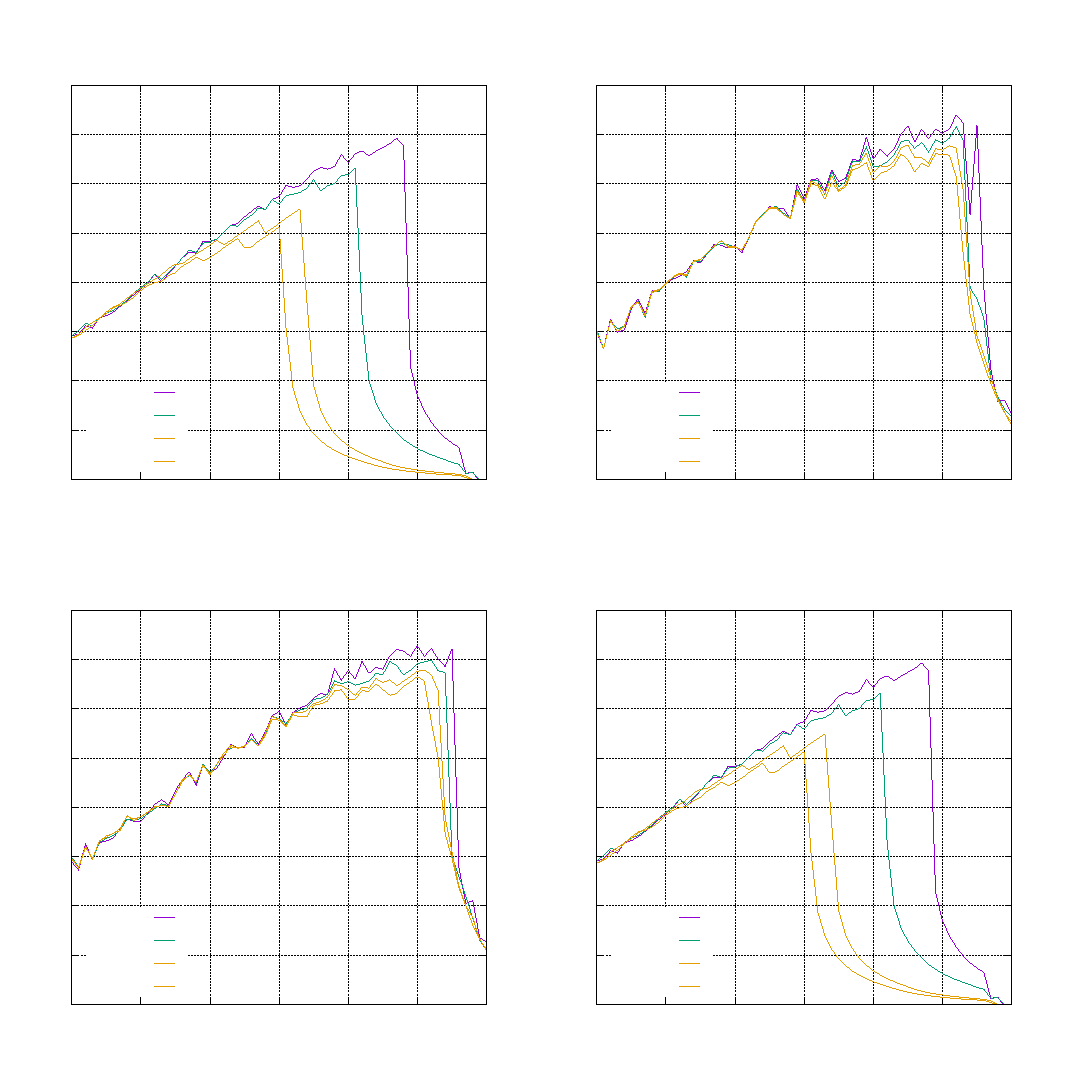
\includegraphics{fourplot}}%
    \gplfronttext
  \end{picture}%
\endgroup
}

	%%% GNUPLOT: LaTeX picture with Postscript
\begingroup
  \makeatletter
  \providecommand\color[2][]{%
    \GenericError{(gnuplot) \space\space\space\@spaces}{%
      Package color not loaded in conjunction with
      terminal option `colourtext'%
    }{See the gnuplot documentation for explanation.%
    }{Either use 'blacktext' in gnuplot or load the package
      color.sty in LaTeX.}%
    \renewcommand\color[2][]{}%
  }%
  \providecommand\includegraphics[2][]{%
    \GenericError{(gnuplot) \space\space\space\@spaces}{%
      Package graphicx or graphics not loaded%
    }{See the gnuplot documentation for explanation.%
    }{The gnuplot epslatex terminal needs graphicx.sty or graphics.sty.}%
    \renewcommand\includegraphics[2][]{}%
  }%
  \providecommand\rotatebox[2]{#2}%
  \@ifundefined{ifGPcolor}{%
    \newif\ifGPcolor
    \GPcolortrue
  }{}%
  \@ifundefined{ifGPblacktext}{%
    \newif\ifGPblacktext
    \GPblacktextfalse
  }{}%
  % define a \g@addto@macro without @ in the name:
  \let\gplgaddtomacro\g@addto@macro
  % define empty templates for all commands taking text:
  \gdef\gplbacktext{}%
  \gdef\gplfronttext{}%
  \makeatother
  \ifGPblacktext
    % no textcolor at all
    \def\colorrgb#1{}%
    \def\colorgray#1{}%
  \else
    % gray or color?
    \ifGPcolor
      \def\colorrgb#1{\color[rgb]{#1}}%
      \def\colorgray#1{\color[gray]{#1}}%
      \expandafter\def\csname LTw\endcsname{\color{white}}%
      \expandafter\def\csname LTb\endcsname{\color{black}}%
      \expandafter\def\csname LTa\endcsname{\color{black}}%
      \expandafter\def\csname LT0\endcsname{\color[rgb]{1,0,0}}%
      \expandafter\def\csname LT1\endcsname{\color[rgb]{0,1,0}}%
      \expandafter\def\csname LT2\endcsname{\color[rgb]{0,0,1}}%
      \expandafter\def\csname LT3\endcsname{\color[rgb]{1,0,1}}%
      \expandafter\def\csname LT4\endcsname{\color[rgb]{0,1,1}}%
      \expandafter\def\csname LT5\endcsname{\color[rgb]{1,1,0}}%
      \expandafter\def\csname LT6\endcsname{\color[rgb]{0,0,0}}%
      \expandafter\def\csname LT7\endcsname{\color[rgb]{1,0.3,0}}%
      \expandafter\def\csname LT8\endcsname{\color[rgb]{0.5,0.5,0.5}}%
    \else
      % gray
      \def\colorrgb#1{\color{black}}%
      \def\colorgray#1{\color[gray]{#1}}%
      \expandafter\def\csname LTw\endcsname{\color{white}}%
      \expandafter\def\csname LTb\endcsname{\color{black}}%
      \expandafter\def\csname LTa\endcsname{\color{black}}%
      \expandafter\def\csname LT0\endcsname{\color{black}}%
      \expandafter\def\csname LT1\endcsname{\color{black}}%
      \expandafter\def\csname LT2\endcsname{\color{black}}%
      \expandafter\def\csname LT3\endcsname{\color{black}}%
      \expandafter\def\csname LT4\endcsname{\color{black}}%
      \expandafter\def\csname LT5\endcsname{\color{black}}%
      \expandafter\def\csname LT6\endcsname{\color{black}}%
      \expandafter\def\csname LT7\endcsname{\color{black}}%
      \expandafter\def\csname LT8\endcsname{\color{black}}%
    \fi
  \fi
    \setlength{\unitlength}{0.0500bp}%
    \ifx\gptboxheight\undefined%
      \newlength{\gptboxheight}%
      \newlength{\gptboxwidth}%
      \newsavebox{\gptboxtext}%
    \fi%
    \setlength{\fboxrule}{0.5pt}%
    \setlength{\fboxsep}{1pt}%
\begin{picture}(5040.00,3772.00)%
    \gplgaddtomacro\gplbacktext{%
      \csname LTb\endcsname%
      \put(396,594){\makebox(0,0)[r]{\strut{}\footnotesize{$0$}}}%
      \csname LTb\endcsname%
      \put(396,954){\makebox(0,0)[r]{\strut{}\footnotesize{$10$}}}%
      \csname LTb\endcsname%
      \put(396,1313){\makebox(0,0)[r]{\strut{}\footnotesize{$20$}}}%
      \csname LTb\endcsname%
      \put(396,1673){\makebox(0,0)[r]{\strut{}\footnotesize{$30$}}}%
      \csname LTb\endcsname%
      \put(396,2032){\makebox(0,0)[r]{\strut{}\footnotesize{$40$}}}%
      \csname LTb\endcsname%
      \put(396,2392){\makebox(0,0)[r]{\strut{}\footnotesize{$50$}}}%
      \csname LTb\endcsname%
      \put(396,2751){\makebox(0,0)[r]{\strut{}\footnotesize{$60$}}}%
      \csname LTb\endcsname%
      \put(396,3111){\makebox(0,0)[r]{\strut{}\footnotesize{$70$}}}%
      \csname LTb\endcsname%
      \put(528,374){\makebox(0,0){\strut{}\footnotesize{$-60$}}}%
      \csname LTb\endcsname%
      \put(1192,374){\makebox(0,0){\strut{}\footnotesize{$-50$}}}%
      \csname LTb\endcsname%
      \put(1856,374){\makebox(0,0){\strut{}\footnotesize{$-40$}}}%
      \csname LTb\endcsname%
      \put(2520,374){\makebox(0,0){\strut{}\footnotesize{$-30$}}}%
      \csname LTb\endcsname%
      \put(3183,374){\makebox(0,0){\strut{}\footnotesize{$-20$}}}%
      \csname LTb\endcsname%
      \put(3847,374){\makebox(0,0){\strut{}\footnotesize{$-10$}}}%
      \csname LTb\endcsname%
      \put(4511,374){\makebox(0,0){\strut{}\footnotesize{$0$}}}%
    }%
    \gplgaddtomacro\gplfronttext{%
      \csname LTb\endcsname%
      \put(88,1852){\rotatebox{-270}{\makebox(0,0){\strut{}\footnotesize{SNR [dB]}}}}%
      \put(2519,154){\makebox(0,0){\strut{}\footnotesize{input [dB]}}}%
      \put(2519,3441){\makebox(0,0){\strut{}\shortstack{16-bit Fixed point \\Cosine $f=0.1$ Q1.15}}}%
      \csname LTb\endcsname%
      \put(1188,1196){\makebox(0,0)[r]{\strut{}\tiny{FFT64}}}%
      \csname LTb\endcsname%
      \put(1188,1042){\makebox(0,0)[r]{\strut{}\tiny{FFT256}}}%
      \csname LTb\endcsname%
      \put(1188,888){\makebox(0,0)[r]{\strut{}\tiny{FFT1024}}}%
      \csname LTb\endcsname%
      \put(1188,734){\makebox(0,0)[r]{\strut{}\tiny{FFT4096}}}%
    }%
    \gplbacktext
    \put(0,0){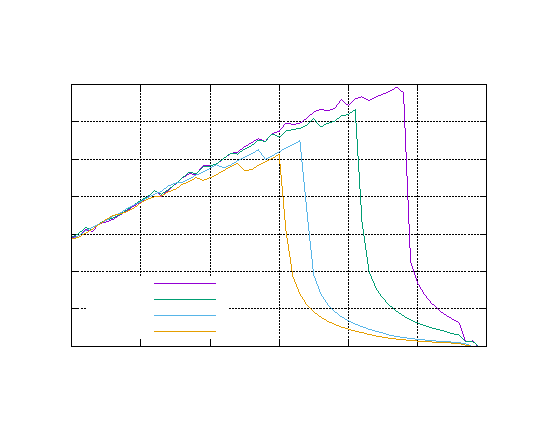
\includegraphics{cosine_DR}}%
    \gplfronttext
  \end{picture}%
\endgroup

	\caption{Output comparison.}
	\label{Fig:COMP}
\end{figure}
First of all it is interesting to see the output of the program with respect to the variation of input signal and FFT size. Figure \ref{Fig:COMP} shows the output of the 16-bit fixed point simulation.\\
One notable aspect is that the input dynamic range of the cosine is more dependent on the FFT size compared to the others. This is probably due to the particular Fourier transform of the cosine, which is composed of only two components. These component are noticeably higher than those that could be found in the FFT of a pure noise signal, and clearly will produce many more saturations.
\subsection{25-bit Decimal Representation}
\label{25BIT}
In order to properly compare the two fixed point representations, the input source needs to be exactly the same( in this case is set as 16 bits of precision). In order to put these 16 bits into a 25-bit numbers without cutting out digits, many different solutions are possible. If we want to keep the same magnitude as the 16-bit version, then a Q1.24 is the only solution, but it is possible to assign more bits to the integer value, such as Q2.23 or Q5.20, down to Q10.15. The results of this comparison are shown in Figure \ref{Fig:25bit} (please note that the input range is different than the others graphs found in this report).\\

As can be seen from the graph, the maximum acceptable input strength increases together with the number of bits of the integer part, topping at 35dB with Q10.15. One less evident but still important aspect is that, apart from saturation, with the same input signal, having more fractional bits produces better results in terms of SNR.

\begin{figure}
	\centering
	\resizebox{1.0\textwidth}{!}{% GNUPLOT: LaTeX picture with Postscript
\begingroup
  \makeatletter
  \providecommand\color[2][]{%
    \GenericError{(gnuplot) \space\space\space\@spaces}{%
      Package color not loaded in conjunction with
      terminal option `colourtext'%
    }{See the gnuplot documentation for explanation.%
    }{Either use 'blacktext' in gnuplot or load the package
      color.sty in LaTeX.}%
    \renewcommand\color[2][]{}%
  }%
  \providecommand\includegraphics[2][]{%
    \GenericError{(gnuplot) \space\space\space\@spaces}{%
      Package graphicx or graphics not loaded%
    }{See the gnuplot documentation for explanation.%
    }{The gnuplot epslatex terminal needs graphicx.sty or graphics.sty.}%
    \renewcommand\includegraphics[2][]{}%
  }%
  \providecommand\rotatebox[2]{#2}%
  \@ifundefined{ifGPcolor}{%
    \newif\ifGPcolor
    \GPcolortrue
  }{}%
  \@ifundefined{ifGPblacktext}{%
    \newif\ifGPblacktext
    \GPblacktextfalse
  }{}%
  % define a \g@addto@macro without @ in the name:
  \let\gplgaddtomacro\g@addto@macro
  % define empty templates for all commands taking text:
  \gdef\gplbacktext{}%
  \gdef\gplfronttext{}%
  \makeatother
  \ifGPblacktext
    % no textcolor at all
    \def\colorrgb#1{}%
    \def\colorgray#1{}%
  \else
    % gray or color?
    \ifGPcolor
      \def\colorrgb#1{\color[rgb]{#1}}%
      \def\colorgray#1{\color[gray]{#1}}%
      \expandafter\def\csname LTw\endcsname{\color{white}}%
      \expandafter\def\csname LTb\endcsname{\color{black}}%
      \expandafter\def\csname LTa\endcsname{\color{black}}%
      \expandafter\def\csname LT0\endcsname{\color[rgb]{1,0,0}}%
      \expandafter\def\csname LT1\endcsname{\color[rgb]{0,1,0}}%
      \expandafter\def\csname LT2\endcsname{\color[rgb]{0,0,1}}%
      \expandafter\def\csname LT3\endcsname{\color[rgb]{1,0,1}}%
      \expandafter\def\csname LT4\endcsname{\color[rgb]{0,1,1}}%
      \expandafter\def\csname LT5\endcsname{\color[rgb]{1,1,0}}%
      \expandafter\def\csname LT6\endcsname{\color[rgb]{0,0,0}}%
      \expandafter\def\csname LT7\endcsname{\color[rgb]{1,0.3,0}}%
      \expandafter\def\csname LT8\endcsname{\color[rgb]{0.5,0.5,0.5}}%
    \else
      % gray
      \def\colorrgb#1{\color{black}}%
      \def\colorgray#1{\color[gray]{#1}}%
      \expandafter\def\csname LTw\endcsname{\color{white}}%
      \expandafter\def\csname LTb\endcsname{\color{black}}%
      \expandafter\def\csname LTa\endcsname{\color{black}}%
      \expandafter\def\csname LT0\endcsname{\color{black}}%
      \expandafter\def\csname LT1\endcsname{\color{black}}%
      \expandafter\def\csname LT2\endcsname{\color{black}}%
      \expandafter\def\csname LT3\endcsname{\color{black}}%
      \expandafter\def\csname LT4\endcsname{\color{black}}%
      \expandafter\def\csname LT5\endcsname{\color{black}}%
      \expandafter\def\csname LT6\endcsname{\color{black}}%
      \expandafter\def\csname LT7\endcsname{\color{black}}%
      \expandafter\def\csname LT8\endcsname{\color{black}}%
    \fi
  \fi
    \setlength{\unitlength}{0.0500bp}%
    \ifx\gptboxheight\undefined%
      \newlength{\gptboxheight}%
      \newlength{\gptboxwidth}%
      \newsavebox{\gptboxtext}%
    \fi%
    \setlength{\fboxrule}{0.5pt}%
    \setlength{\fboxsep}{1pt}%
\begin{picture}(5040.00,3772.00)%
    \gplgaddtomacro\gplbacktext{%
      \csname LTb\endcsname%
      \put(396,594){\makebox(0,0)[r]{\strut{}\footnotesize{$50$}}}%
      \csname LTb\endcsname%
      \put(396,1097){\makebox(0,0)[r]{\strut{}\footnotesize{$60$}}}%
      \csname LTb\endcsname%
      \put(396,1601){\makebox(0,0)[r]{\strut{}\footnotesize{$70$}}}%
      \csname LTb\endcsname%
      \put(396,2104){\makebox(0,0)[r]{\strut{}\footnotesize{$80$}}}%
      \csname LTb\endcsname%
      \put(396,2608){\makebox(0,0)[r]{\strut{}\footnotesize{$90$}}}%
      \csname LTb\endcsname%
      \put(396,3111){\makebox(0,0)[r]{\strut{}\footnotesize{$100$}}}%
      \csname LTb\endcsname%
      \put(528,374){\makebox(0,0){\strut{}\footnotesize{$-30$}}}%
      \csname LTb\endcsname%
      \put(984,374){\makebox(0,0){\strut{}\footnotesize{$-20$}}}%
      \csname LTb\endcsname%
      \put(1440,374){\makebox(0,0){\strut{}\footnotesize{$-10$}}}%
      \csname LTb\endcsname%
      \put(1896,374){\makebox(0,0){\strut{}\footnotesize{$0$}}}%
      \csname LTb\endcsname%
      \put(2351,374){\makebox(0,0){\strut{}\footnotesize{$10$}}}%
      \csname LTb\endcsname%
      \put(2807,374){\makebox(0,0){\strut{}\footnotesize{$20$}}}%
      \csname LTb\endcsname%
      \put(3263,374){\makebox(0,0){\strut{}\footnotesize{$30$}}}%
      \csname LTb\endcsname%
      \put(3719,374){\makebox(0,0){\strut{}\footnotesize{$40$}}}%
    }%
    \gplgaddtomacro\gplfronttext{%
      \csname LTb\endcsname%
      \put(-44,1852){\rotatebox{-270}{\makebox(0,0){\strut{}\footnotesize{SNR [dB]}}}}%
      \put(2123,154){\makebox(0,0){\strut{}\footnotesize{input [dB]}}}%
      \put(2123,3441){\makebox(0,0){\strut{}\shortstack{Input Dynamic Range\\16QAM Q1.15 FFT256}}}%
      \csname LTb\endcsname%
      \put(4181,3001){\makebox(0,0)[r]{\strut{}\tiny{Q10.15}}}%
      \csname LTb\endcsname%
      \put(4181,2781){\makebox(0,0)[r]{\strut{}\tiny{Q9.16}}}%
      \csname LTb\endcsname%
      \put(4181,2561){\makebox(0,0)[r]{\strut{}\tiny{Q8.17}}}%
      \csname LTb\endcsname%
      \put(4181,2341){\makebox(0,0)[r]{\strut{}\tiny{Q7.18}}}%
      \csname LTb\endcsname%
      \put(4181,2121){\makebox(0,0)[r]{\strut{}\tiny{Q6.19}}}%
      \csname LTb\endcsname%
      \put(4181,1901){\makebox(0,0)[r]{\strut{}\tiny{Q5.20}}}%
      \csname LTb\endcsname%
      \put(4181,1681){\makebox(0,0)[r]{\strut{}\tiny{Q4.21}}}%
      \csname LTb\endcsname%
      \put(4181,1461){\makebox(0,0)[r]{\strut{}\tiny{Q3.22}}}%
      \csname LTb\endcsname%
      \put(4181,1241){\makebox(0,0)[r]{\strut{}\tiny{Q2.23}}}%
      \csname LTb\endcsname%
      \put(4181,1021){\makebox(0,0)[r]{\strut{}\tiny{Q1.24}}}%
    }%
    \gplbacktext
    \put(0,0){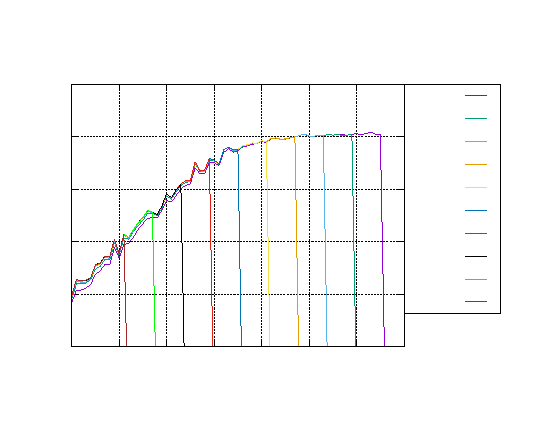
\includegraphics{q25shift}}%
    \gplfronttext
  \end{picture}%
\endgroup
}
	\caption{Comparison of 25-bit fixed point representations.}
	\label{Fig:25bit}
\end{figure}

\section{Code}
\noindent\begin{minipage}{.45\textwidth}
\begin{lstlisting}[caption=complex.h - original,label={CODE:CMXO},frame=tlrb, language=C]{Name}
struct complex{
    double r;
    double i;
    };

struct complex16{
    short r;
    short i;
};

struct complex32{
    int r;
    int i;
};
    \end{lstlisting}
\end{minipage}\hfill
\begin{minipage}{.45\textwidth}
    \begin{lstlisting}[caption=complex.h - modified, label={CODE:CMXM}, frame=tlrb, language=C]{Name}
struct complex{
    double r;
    double i;
};

struct complex16{
    int16_t r;
    int16_t i;
};

struct complex32{
    int32_t r;
    int32_t i;
};
    \end{lstlisting}
\end{minipage}
\newpage
\begin{lstlisting}[caption=fft.c - twiddle factors, label={CODE:TWID},frame=tlrb, language=C]{Name}
void twiddle(struct complex *W, int N, double stuff){
    W->r=cos(stuff*2.0*PI/(double)N);
    W->i=-sin(stuff*2.0*PI/(double)N);
}

void twiddle_fixed(struct complex16 *W, int N, double stuff){
    W->r=(int16_t)(32767.0*cos(stuff*2.0*PI/(double)N));
    W->i=(int16_t)(-32768.0*sin(stuff*2.0*PI/(double)N));
    }

void twiddle_fixed_Q17(struct complex32 *W, int N, double stuff){
    W->r=(int32_t)(131071.0*cos(stuff*2.0*PI/(double)N));
W->i=(int32_t)(-131072.0*sin(stuff*2.0*PI/(double)N));
}
\end{lstlisting}

\noindent\begin{minipage}{.45\textwidth}
	\begin{lstlisting}[caption=fft.c - bit reordering - original, label={CODE:REORDERO}, frame=tlrb, language=C]{Name}
void bit_r4_reorder_fixed_Q15(
struct complex16 *W,
int N,
char scale)
{
  int bits, i, j, k;
  short tempr, tempi;






  for (i=0; i<MAXPOW; i++)
    if (pow_2[i]==N) bits=i;

  for (i=0; i<N; i++){
    j=0;
    for (k=0; k<bits; k+=2){
      ...
    }

    if (j>i){
      tempr=W[i].r>>scale;
      tempi=W[i].i>>scale;
      W[i].r=W[j].r>>scale;
      W[i].i=W[j].i>>scale;
      W[j].r=tempr;
      W[j].i=tempi;
    }
  }
}
\end{lstlisting}
\end{minipage}\hfill
\begin{minipage}{.45\textwidth}
\begin{lstlisting}[caption=fft.c - bit reordering - modified, label={CODE:REORDERM}, frame=tlrb, language=C]{Name}
void bit_r4_reorder_fixed_Q15(
struct complex16 *W,
int N,
char scale)
{
  int bits, i, j, k;
  int16_t tempr, tempi;

  for(i=0; i<N; i++){
    W[i].r=W[i].r>>scale;
	W[i].i=W[i].i>>scale;
	}

  for (i=0; i<MAXPOW; i++)
    if (pow_2[i]==N) bits=i;

  for (i=0; i<N; i++){
    j=0;
   	for (k=0; k<bits; k+=2){
   	  ...
   	}

    if (j>i){
      tempr=W[i].r;
      tempi=W[i].i;
      W[i].r=W[j].r;
      W[i].i=W[j].i;
      W[j].r=tempr;
      W[j].i=tempi;
    }
  }
}
    \end{lstlisting}
\end{minipage}    
\newpage
\begin{lstlisting}[caption=fft.c - radix4 Q15,label={CODE:RADIX4},frame=tlrb, language=C]{Name}
void radix4_fixed_Q15(struct complex16 *x,   // Input in Q15 format
int N,                 // Size of FFT
unsigned char *scale,  // Pointer to scaling schedule
unsigned char stage)   // Stage of fft
{
int    n2, k1, N1, N2;
struct complex16 W, bfly[4];

N1=4;
N2=N/4;

// Do 4 Point DFT
for (n2=0; n2<N2; n2++){
    // scale Butterfly input
x[n2].r          >>= scale[stage];
...
x[(3*N2) + n2].i >>= scale[stage];

// Radix 4 Butterfly
bfly[0].r = SAT_ADD16(  SAT_ADD16(x[n2].r, x[N2 + n2].r) ,
            SAT_ADD16(x[2*N2+n2].r, x[3*N2+n2].r));
bfly[0].i = SAT_ADD16(  SAT_ADD16(x[n2].i, x[N2 + n2].i) ,
            SAT_ADD16(x[2*N2+n2].i, x[3*N2+n2].i));
bfly[1].r = SAT_ADD16(  SAT_ADD16(x[n2].r, x[N2 + n2].i) ,
           -SAT_ADD16(x[2*N2+n2].r, x[3*N2+n2].i));
bfly[1].i = SAT_ADD16(  SAT_ADD16(x[n2].i, -x[N2 + n2].r) ,
            SAT_ADD16(-x[2*N2+n2].i, x[3*N2+n2].r));
bfly[2].r = SAT_ADD16(  SAT_ADD16(x[n2].r, -x[N2 + n2].r) ,
            SAT_ADD16(x[2*N2+n2].r, -x[3*N2+n2].r));
bfly[2].i = SAT_ADD16(  SAT_ADD16(x[n2].i, -x[N2 + n2].i) ,
            SAT_ADD16(x[2*N2+n2].i, -x[3*N2+n2].i));
bfly[3].r = SAT_ADD16(  SAT_ADD16(x[n2].r, -x[N2 + n2].i) ,
            SAT_ADD16(-x[2*N2+n2].r, x[3*N2+n2].i));
bfly[3].i = SAT_ADD16(  SAT_ADD16(x[n2].i, x[N2 + n2].r) ,
            SAT_ADD16(-x[2*N2+n2].i, -x[3*N2+n2].r));

// In-place results
x[n2].r = bfly[0].r;
x[n2].i = bfly[0].i;

for (k1=1; k1<N1; k1++){
    twiddle_fixed(&W, N, (double)k1*(double)n2);
    x[n2 + N2*k1].r = SAT_ADD16( FIX_MPY(bfly[k1].r, W.r) ,
                     -FIX_MPY(bfly[k1].i, W.i) );
    x[n2 + N2*k1].i = SAT_ADD16( FIX_MPY(bfly[k1].i, W.r) ,
                      FIX_MPY(bfly[k1].r, W.i) );
}
}

// Don't recurse if we're down to one butterfly
if (N2!=1)
for (k1=0; k1<N1; k1++){
    radix4_fixed_Q15(&x[N2*k1], N2,scale,stage+1);
}
}
\end{lstlisting}


\end{document}
